\documentclass{llncs}

\usepackage{graphicx}
\usepackage{amsmath}

\newcommand{\field}[1]{{\mathbf{#1}}}

\begin{document}

\frontmatter
\pagestyle{headings}

%\tableofcontents

\mainmatter

\title{Automatic Differentiation of C++ Codes for Large-Scale Scientific Computing}
\titlerunning{AD of C++ Codes}

\author{Roscoe A. Bartlett \and David M. Gay \and Eric T. Phipps}
\authorrunning{Bartlett et al.}

\tocauthor{Roscoe Bartlett, David Gay, and Eric Phipps (Sandia National Laboratories)}

\institute{Sandia National Laboratories\footnote{Sandia is a multiprogram laboratory operated by Sandia Corporation, a Lockheed Martin Company, for the United States Department of Energy under Contract DE-AC04-94AL85000.}, Albuquerque NM 87185, USA}
%This is SAND2005-7816C.

\maketitle

\begin{abstract}
We discuss computing first derivatives for models based on elements,
such as large-scale
finite-element PDE discretizations, implemented in the C++ programming
language.  We use a hybrid technique of automatic differentiation (AD)
and manual assembly, with local element-level derivatives computed via AD and
manually summed into the global derivative.  C++ templating and
operator overloading work well for both forward- and reverse-mode derivative
computations.
We found that AD
derivative computations compared favorably in time to finite differencing
for a scalable
finite-element discretization of a
convection-diffusion problem in two dimensions.
\end{abstract}

Computing derivatives is ubiquitous in scientific computing; examples
include algorithms for nonlinear equation solving, optimization, stability analysis,
and implicit time integration.  Computing derivatives quickly and
accurately improves both the efficiency and
robustness of these numerical algorithms, particularly in the presence
of ill-conditioning.  In this paper, we discuss computing first
derivatives of element-based models implemented in ANSI/ISO C++.  We
use the term ``element'' in a broad sense to encompass any model whose
computation consists of repeated evaluations of a small set of
functions, each involving relatively few of the variables
of the overall problem.
Many classes of models fall into this category, including
finite-element and finite-volume PDE discretizations and network
models.  We use a hybrid technique of automatic differentiation (AD)
and manual assembly similar
to~\cite{Abate2001IAw,Tijskens2002ADf} to carry out the model evaluation and
derivative computation one element at a time.  This
decomposition is discussed in more detail in
Section~\ref{sect:element}, which generalizes the ideas
in~\cite{Tijskens2002ADf} to general element-based models and
additionally describes how to compute the global adjoint.

We focus on ANSI/ISO C++ codes because much
modern scientific code development is done in C++.
Since no source transformation tools for C++ were available to
us, we used C++ operator overloading
to implement AD for computing the element-level derivatives.
We assume the
reader is familiar with AD and the
methods for implementing it; see~\cite{Griewank2000EDP} for a good
introduction to these concepts.  We used two
separate AD packages: the public domain package Fad~\cite{Aubert2001ADi} for
forward-mode AD and our own reverse-mode package Rad~\cite{Gay2005SDf}.
We sought to determine if AD based on
operator overloading could be incorporated effectively into a
large, evolving scientific application code and whether the resulting
derivative calculations would be efficient enough for scientific use,
particularly for reverse-mode gradient evaluations.  We
applied this approach to a large-scale finite-element simulation code called Charon,
developed at Sandia
National Laboratories for reacting fluid flows and
semiconductor device simulations.  Details of the implementation are
presented in Section~\ref{sect:AD}, along with a discussion of
difficulties we encountered.  To
assess efficiency, in Section~\ref{sect:charon} we report
flop counts and run times for Jacobian and Jacobian-transpose
products and finite differences on a small convection-diffusion
problem.

We believe the work presented here to be novel in a number of ways.
While there have been several successful applications of automatic
differentiation to Fortran-based scientific codes using source
transformation, we knew of no experience with this in large C++
codes.  Successfully incorporating AD by operator
overloading and templating into such an application code is,
we believe, both nontrivial
and new, and the process we used merits discussion.  While
computing element derivatives was used as motivation for development
of the Rad tool presented in~\cite{Gay2005SDf}, the work here
represents the first measurement of the performance of Rad in a real
scientific code.

\section{Computing Derivatives of Element-Based Models}
\label{sect:element}

We are concerned with evaluating and computing derivatives of a
continuously differentiable, vector valued function
%\begin{displaymath}
%\label{eq:global_residual}
$f: \field{R}^n \rightarrow \field{R}^m,$
%\end{displaymath}
in which $m$ and $n$ may be large,
on the order of millions, and in which $f(x)$ is the sum
\begin{equation}\label{eq:f-element-sum}
f(x) = \sum_{i=1}^{N} Q_i^T e_{k_i}(P_i x)
\end{equation}
of a large number $N$ of elements taken from a small
set $\{ e_k \}$ of element
functions $e_k : \field{R}^{n_k}\rightarrow\field{R}^{m_k}$ where
typically each $n_k$, $m_k$ are on the order of 10 to 100.
The matrices $P_i \in \field{R}^{n_{k_i} \times n}$
and $Q_i \in \field{R}^{m_{k_i} \times m}$ map global vectors
to the local element domain and range spaces respectively.
Often we seek
$x$ such that $f(x)=0$, so we call $f(x)$ the
global residual.

In some applications, such as the one we discuss in Section \ref{sect:charon},
it is convenient to
deal with ``interior'' and ``boundary'' elements separately, with the boundary
elements modifying or replacing some values computed by the interior elements.
In effect, we compute $f(x) = (I - S^T S) f_I(x) + S^T f_B(x)$, where
$(I - S^T S)$ is a projection matrix that replaces some components of the sum $f_I(x)$
of the interior elements by zeros.  We suppress this extra complexity in what follows,
since it is orthogonal to the other issues we discuss.

Given (\ref{eq:f-element-sum}), we can clearly compute
the global Jacobian $J = \partial f/\partial x$ and
adjoint $\bar{J} = w^T J$ element-wise:
\begin{equation*}
\frac{\partial f}{\partial x} = \sum_{i=1}^{N} Q_i^T J_{k_i} P_i, \qquad
w^T\frac{\partial f}{\partial x} = \sum_{i=1}^{N} (Q_i w)^T J_{k_i} P_i
\end{equation*}
where
$J_{k_i} = \partial e_{k_i}/\partial P_i x$ is the Jacobian
matrix of $e_{k_i}$.

With these decompositions, we have translated the difficult task of
computing the global Jacobian and adjoint into a series of much
smaller computations on elements.  In principle,
any method can be used to compute these element-level derivatives:
AD, symbolic differentiation, or finite
differencing.  This task is well suited to AD
for several reasons.  First, each element function $e_k$
has only a few independent and dependent variables,
often around ten and at most a few hundred, so the element
Jacobians $J_i = \partial e_{k_i} / \partial P_i x$
can be treated as dense matrices, and there is no need to use sparse AD techniques.
Second, each element computation is fairly simple,
involving only a few operations per variable.  Thus
the memory burden of reverse-mode AD is reasonable and
checkpointing is not generally required.  Third, all parallel
communication occurs during gathering of the local variables and
scattering of the results to the global residuals/derivatives, which
means it is not necessary to differentiate through parallel
communications.  Lastly, the structure of the derivative assembly
closely mirrors the residual assembly, particularly when we implement
AD via templating and operator overloading.  This allows much of the same code
for the residual evaluation to be reused for the derivative computation,
as discussed next.

\section{Computing Element Derivatives Via AD in C++}
\label{sect:AD}

We turn now to some practical details of implementing AD via
operator overloading in the large, element-based scientific C++ code
Charon, developed at Sandia National Laboratories
for simulation of reacting fluid flows and
semiconductor devices.  Our goals were to determine if
AD based on operator overloading could be effectively incorporated into
such an application code and whether the resulting derivative
calculations would be efficient enough for production use.

To compute derivatives using forward AD, there are many publicly
available C++ tools that in principle could be applied.  We chose the
Fad~\cite{Aubert2001ADi} package because of its reputation for
efficiency, flexibility, and simplicity.  Fad uses expression
templates to eliminate much of the overhead normally associated with
operator overloading.  However, because the exact physics Charon is
simulating is not known until run time, we were forced to use the
version of Fad that uses dynamic memory allocation of the derivative array.

For reverse-mode derivative computations, we chose the Rad~\cite{Gay2005SDf}
package, which is designed precisely for element gradient computations.
Rad records just enough detail during an element evaluation to
permit efficient reverse accumulation of the element gradient;
Rad retains scratch memory, immediately reusing it when evaluation
of the next element begins.

To use these tools in Charon, we found
C++ templating highly effective for computing the element functions $e_k$.
In brief, we changed scalar floating-point types (\texttt{double}
or \texttt{float}) to templated types in
all C++ classes used in computing the $e_k$.  Then by instantiating
the resulting templated classes on the floating-point type, we get
the original element evaluations, and by instantiating on the AD
types, we compute both the element functions and their derivatives.
We also templated the initialization
and post-processing classes that gather
and scatter to and from local variables (i.e., that compute $P_i x$
and $Q_i^T e_{k_i}$, given $e_{k_i}$).  In addition to
gathering and scattering, the AD specializations
initialize the seed matrix (for Fad) and extract the element derivatives.

By providing other
AD types, one could obtain many other kinds of derivatives,
such as Hessian-vector products, and Taylor polynomials.  This results in major
savings in code development time, since only one templated residual
computation needs to be written and maintained.  We believe this
approach is significantly more suitable to a large, evolving
application code than the standard approach of copying the
undifferentiated source and manually changing the type.  Templating makes it impossible for the differentiated source code
to become out of sync with the undifferentiated source, and forces the
developer to think about how the source should be differentiated at
development time.

Overall, we found our approach to be an effective way to use AD
in Charon, but we did encounter some difficulties.
First, interfacing the templated functions and classes for computing
the $e_k$ to the rest of the non-templated application code in a
manner that easily allows new template types to be added to the
application code required some significant C++ software engineering.
In brief, we used container classes for storing instantiations of
each templated class.  This allows ``glue'' code to interface
template and non-template code in a manner independent of the
choices of AD data types.

Second, most C++ application codes use libraries written in
other languages, such as Fortran.  For example, Charon uses
Chemkin~\cite{Chemkin} to simulate chemical reactions appearing
in elements.  A simple way to deal with this
is to provide a templated interface class that has
specializations for each AD type.  These specializations extract
derivative values out of the C++ classes and then compute derivatives
of the Fortran source by whatever mechanism is available.  In Charon,
we have a forward-mode differentiated version of the Chemkin source
provided by  ADIFOR 2.0~\cite{Bischof1996A2A}, and this version is used by both
the Fad and Rad Charon/Chemkin interface classes.  We
plan later to make reverse-mode differentiated Chemkin source available for
the Rad specialization, provided by one or more of OpenAD~\cite{Utke2004OAI},
ADIFOR 3.0, or Tapenade~\cite{tapenade}.

Third, templating the application code classes can lengthen
the time taken to compile the application significantly.
Since definitions of templated functions and classes
must be available at the time they are instantiated, typically when
they are first referenced in a source file, the template
definitions are often placed in header files along with the
declarations.  This results in code-bloat, and increased compile times
since all of the template definitions must be recompiled in each
translation unit.  This additional compile time
was probably the single largest hurdle to
effectively incorporating AD into Charon.  To cope, we
split the header file for a templated class into three files, a
declaration header, an implementation header, and a source file
that includes both and explicitly instantiates the class on all AD
types via a preprocessor macro.  This drastically reduces the
recompilation time of the application code, putting it on par with
the original un-templated code.

Finally, passive variables gave us trouble with
incorporating reverse-mode AD into Charon.  Such ``variables''
act as constants, but are stored as AD types for
flexibility.  Since Charon supports multiple physics,
it is hard in some parts of the code to know whether a quantity,
say temperature, is a constant or an unknown being solved for.
To avoid storing the
temperature as a passive variable, we could provide
two instantiations of the element functions, one for when
temperature is an unknown
(AD type) and one for when it is constant (a floating-point type).
This would be necessary
for any quantity that could be constant or variable, yielding a
combinatorial explosion of template instantiations.
To avoid this explosion, we always store potentially active variables
as active.
For reverse AD, this requires us to tell Rad which of these active
variables are really constants (since they will not be reinitialized), so
Rad can store them in memory that is not recycled at the beginning
of each element evaluation.  We think we can find a place in
Charon where all passive variables are known, so Rad could be
told before the first function evaluation to treat them as constants,
but so far we have pursued more ad-hoc (and less satisfactory) approaches.
Currently we use traits to mark passive variables as
constants, but this requires
finding all potentially passive variables, a daunting task that is
unlikely to be maintainable.
Another approach would be
to assume a variable is constant until it is reinitialized and only to
reuse memory for such non-constants.  We believe this would
substantially reduce Rad's efficiency, but it is an approach that
would be helpful for debugging, and we are looking into it.

\section{An Example Convection-Diffusion Problem}
\label{sect:charon}

We now compare costs of alternative derivative computations
in a
small, two dimensional reacting convection-diffusion problem implemented in
Charon.  Since we compute derivatives element-wise, the size of
the AD computation is proportional to the degrees-of-freedom (DOF)
per element, so we study how the costs of the Jacobian and
adjoint computations scale with the DOF.

Our test problem has
a two dimensional rectangular domain $\Omega$ of width 2 and
height 1 containing an ideal fluid with unit density and
constant but spatially varying fluid velocity $\mathbf{u}$.  The fluid
contains $N$ chemical species $X_1,\dots,X_N$, with mass fractions
$Y_1,\dots,Y_N$, unit molecular weights and unit diffusion
coefficients.  The chemical
species undergo the following hypothetical chemical reactions:
\begin{math}
  2 X_j \rightleftharpoons X_{j-1} + X_{j+1}, \; j=2,\dots,N-1,
\end{math}
with both unit forward and reverse rate constants.  For each reaction $j$,
the rate of progress for that reaction, $q_j$, satisfies
\begin{displaymath}
  q_j = [X_j]^2 - [X_{j-1}][X_{j+1}] = Y_j^2 - Y_{j-1}Y_{j+1}, \quad
  j=2,\dots,N-1.
\end{displaymath}
Then the production rate
$\dot{\omega}_j$ of chemical species $X_j$ is
$\dot{\omega}_j = q_{j-1} - 2 q_j + q_{j+1}$ for $j=3,\dots,N-2$,
with $\dot{\omega}_1 = q_2$, $\dot{\omega}_2 = -2 q_2 + q_3$, and
$\dot{\omega}_{N-1} = q_{N-2} - 2 q_{N-1}$.
The partial differential equations governing the
mass fractions of the $N$ species are given by
\begin{equation}
\label{eq:pde}
\begin{split}
  \frac{\partial Y_j}{\partial t} + \mathbf{u}\cdot\nabla Y_j +
  \nabla^2 Y_j &= \dot{\omega}_j, \quad j=1,\dots,N-1 \\
  \sum_{j=1}^N Y_j &= 1.
\end{split}
\end{equation}
Charon uses bilinear
basis functions and quadrangle finite elements in a
Galerkin,
least-squares discretization~\cite{hufh:89}.
Each element has a side
length of 0.1, giving 200 total elements and four nodes per element.

Normally we would use
Chemkin to compute the production rates
$\dot{\omega}_j$, but to study the
efficiency of the operator overloading approach, we used hand-coded C++
instead.
We ignored spatial boundary conditions on the domain $\Omega$, since
they are not
relevant to the computational complexity of the
residual, Jacobian, and adjoint computations.  To avoid complications
in time integration, we made
this a steady-state problem by setting $\partial Y_j/\partial t = 0$,
$j=1,\dots,N$.  While these simplifications give a highly contrived test problem that is not
physically meaningful, it does have two important qualities.  First,
structurally it is qualitatively similar to many of the PDE problems
to which Charon is applied, and second we can easily vary
the number of unknowns to see how the cost of AD scales.

\begin{figure}[tb]
  \begin{center}
    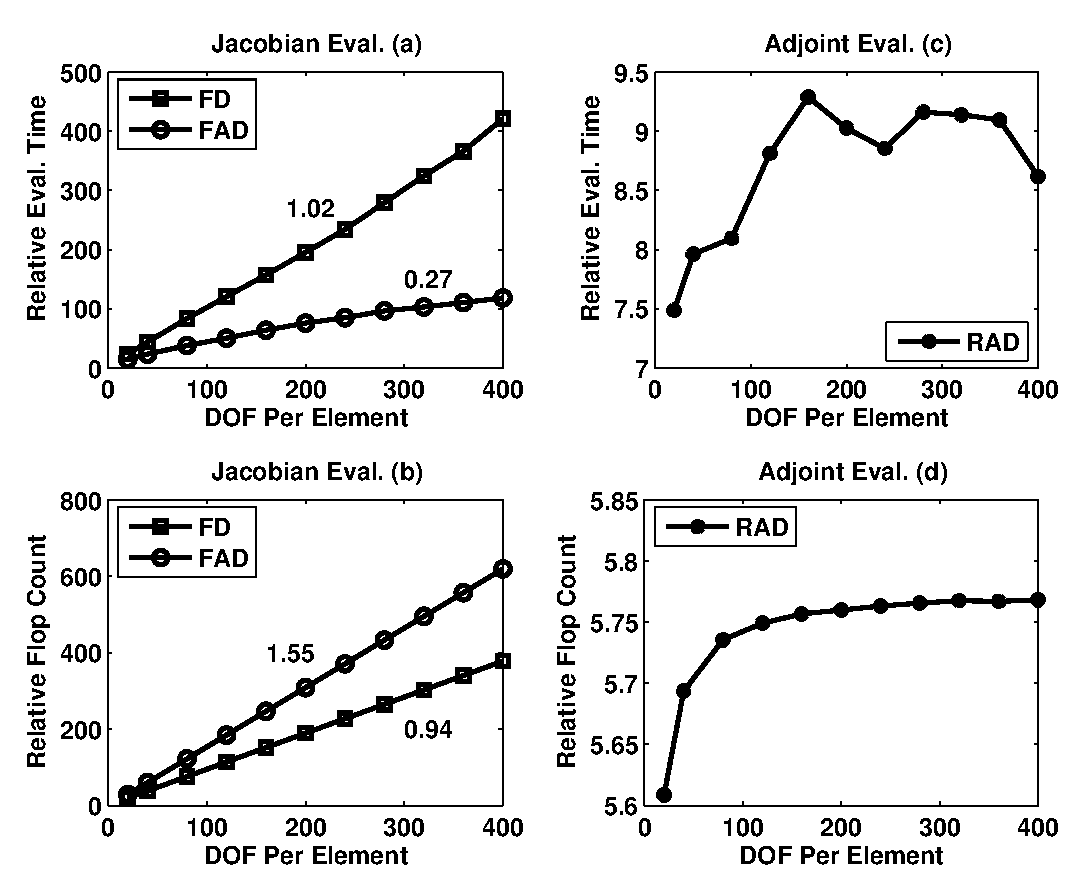
\includegraphics[width=10cm]{perf.eps}
    \caption{Jacobian and adjoint evaluations versus
    degrees of freedom ($DOF = 4 \; \times$ number of
    species). ({\bf a}) Relative Jacobian computation times.
    ({\bf b}) Relative Jacobian flop counts.  ({\bf c})
    Relative adjoint ($w^T J$) times. ({\bf d}) Relative adjoint flop counts}
    \label{figure:performance}
  \end{center}
\end{figure}
We computed ratios of Jacobian to residual evaluation time for the
discretized form of \eqref{eq:pde}, using both
Fad and finite differencing to compute the element-level Jacobians.
Figure~\ref{figure:performance}(a) shows how these ratios
vary with the
degrees-of-freedom per element.
We computed corresponding floating-point operation (flop) count ratios,
which are shown in Figure~\ref{figure:performance}(b).
(Templating made getting the flop counts easy.)
We used gcc 3.4.4 with $\texttt{-O2}$ optimization on a 3.2 Ghz dual-processor (Xenon)
workstation having 2 GB of RAM and a 512 KB level-1 cache, running Fedora Core 3
Linux.
Note that while an individual element computation may fit entirely in cache,
the entire 200 element residual evaluation does not.
As expected, both the time and flop-count ratios scaled nearly linearly with
the DOF per element, with slopes of about 0.27 and 1.55
respectively.  While Fad Jacobian computations used
roughly 50\% more operations than finite differences, Fad
was more than three times faster.  The exact cause of this timing difference is unclear, but is
likely related to improved data locality due to vectorization of the
forward mode.  A relative flop
count slope slightly
above 1.5 is not unexpected~\cite{Griewank2000EDP}.
Fad recomputes each operation once for every
derivative component, to give the compiler a
chance to optimize temporary template objects away.  We are investigating ways
to cache operation results while still letting the compiler
optimize temporaries away, in hopes
of making Fad even more efficient.

Relative times and flop counts for an adjoint ($w^T J$) computation appear in
Figures~\ref{figure:performance}(c) and \ref{figure:performance}(d).  The adjoint computation took
between 7.5 and 9.5 times longer than the residual computation, but
used only about 5.6 to 5.8 times as many operations.  Compared with Fad,
Rad had a larger ratio
of time to flops, because of the extra memory overhead of reverse-mode AD.
However, this still seems reasonably
efficient:  computing an adjoint with 400
DOF is ten times faster than computing the full Jacobian using
Fad and multiplying by the transpose.

\section{Summary and Conclusions}
\label{sect:summary}

Our tests covered a range of 20 to 400 DOF per element,
which encompasses the problem
sizes normally seen in finite-element application codes.  Again, since the derivatives
are computed element-wise, it is this dimension that dictates the
difficulty of the AD problem, not the number of elements or global
number of unknowns.  Thus for PDE discretizations with up to millions
of unknowns, we have shown that forward-mode AD via Fad is a highly
efficient method for computing the global Jacobian, more
efficient than finite differencing and with better scaling to larger
numbers of PDE equations.  In fact Charon recently computed a
transient simulation of the electric current in a finite element
discretization of a bipolar junction transistor with
more than 2.7 million elements on 128 processors, leveraging the Fad
Jacobian computation for implicit time integration.
We also found that Rad provides
reverse-mode derivative computations with reasonable efficiency,
which makes gradients available for use in optimization and sensitivity analysis.

We are highly encouraged by both the efficiency of forward and reverse
mode AD in C++ codes, and by our experiences with implementation via
templating.  The Fad Jacobian computation is much faster
than conventional finite differencing and provides analytic derivatives as
well.  Templating allows the code developer to write and maintain one
version of source code that has analytic derivatives available
essentially for free.  Many different derivative
quantities then become available, which should enable development and use of advanced
nonlinear solver, optimization, time integration, stability analysis,
and uncertainty quantification algorithms.  We successfully
overcame all hurdles encountered in templating Charon,
and templating is now a permanent feature of the code.  All new code
development of Charon relating to element computations is templated,
so analytic derivatives will always be available for any new features
that are added.  Charon has become an integral component of many
important Sandia projects that require computational simulation and
analysis, in no small part due to availability of analytic derivatives
and the advanced algorithms they enable.

\bibliographystyle{splncs}
\bibliography{paper}

\end{document}
